\documentclass[conference]{IEEEtran}

% Language setting
% Replace `english' with e.g. `spanish' to change the document language
\usepackage[spanish]{babel}

% Useful packages
\usepackage{amsmath}
\usepackage{graphicx}
\usepackage{url}

% Title and author info
\title{Pokemon-API Prototype}
\author{\IEEEauthorblockN{Juan David Cotacio Sánchez}}

\begin{document}
\maketitle

\begin{abstract}
Your abstract.
\end{abstract}

\section{Introducción}
En un mundo donde la nostalgia se fusiona con la innovación, nuestro proyecto Pokémon-API emerge como un homenaje moderno a una de las franquicias más queridas en la historia de los videojuegos: Pokémon. Utilizando tecnologías como CSS, HTML, JavaScript, jQuery ,Artyom y Boostrap hemos creado una experiencia interactiva que transporta a los usuarios a través del universo Pokémon de una manera única y emocionante.


\subsection{Como empezar el prototipo}

Para la creación de este prototipo empece en como podia implementar estas tecnologias, para la inclusión de esta herramientas empece por crear un HTML y CSS a la vez además de importar las librerias que vamos a usar.
\begin{figure}[h] % Aquí comienza la inclusión de la imagen
    \centering
    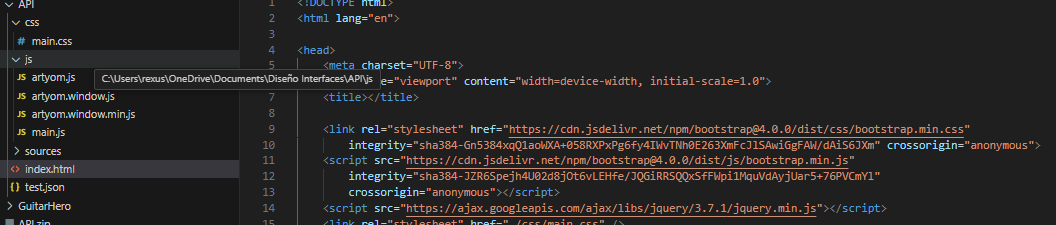
\includegraphics[width=0.5\textwidth]{images/Librerias.png} % Reemplaza 'ruta/de/la/imagen' por la ruta de tu imagen
    \caption{Importación de librerias}
    \label{fig:mi_imagen}
\end{figure}

\subsection{Como se incluyo el CSS, HTML y Boostrap}
Primero empece a crear una estructura en mi HTML para darle el espacio, cree un contenedor general que iba almacenar mis botones y imagenes cabe recalcar que estos botones y barra busqueda son traidos de Boostrap, entonces ya traen un diseño por defecto pero aun así se necesita CSS con su respectiva class y id, para poder modificar su posición, tamaño o color.

En mi css quise añadir las respectivas imagenes de cada una de las cosas que estaba añadiendo en mi HTML, para darle posición y tamaños, en nuestra hoja de estilos lo mas destacable es el manejo de error 404, unos de los problemas que se me presento el de que el error no apareciera apenas se cargara la pagina entonces use la función "display: none;" el cual va ocultar en la pantalla mientras carga la pagina pero aun así se necesitaba manejar logica en JavaScript para poder manejar el error.

\begin{figure}[h] % Aquí comienza la inclusión de la imagen
    \centering
    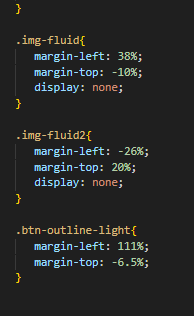
\includegraphics[width=0.2\textwidth]{images/Manejo del error 404.png} % Reemplaza 'ruta/de/la/imagen' por la ruta de tu imagen
    \caption{Uso del "display: none;" }
    \label{fig:mi_imagen}
\end{figure}
\subsection{Acercamiento con la API}
Para usar los conceptos de API, es necesario realizar con algo ya creado e implementarlo en nuestro proyecto, así fue como se llego Poke-API, esta contiene datos destacables de la famosa seria Pokemon, algunas de estos datos son: nombre, habilidades, imagenes o el tipo de este mismo. 

Asi nuestra Pokedex se iba generar de forma dinamica y sencilla pues no se necesitara añadirlo de forma rustica, además de nuevos conceptos como son los Archivos JSON. 

\begin{figure}[h] % Aquí comienza la inclusión de la imagen
    \centering
    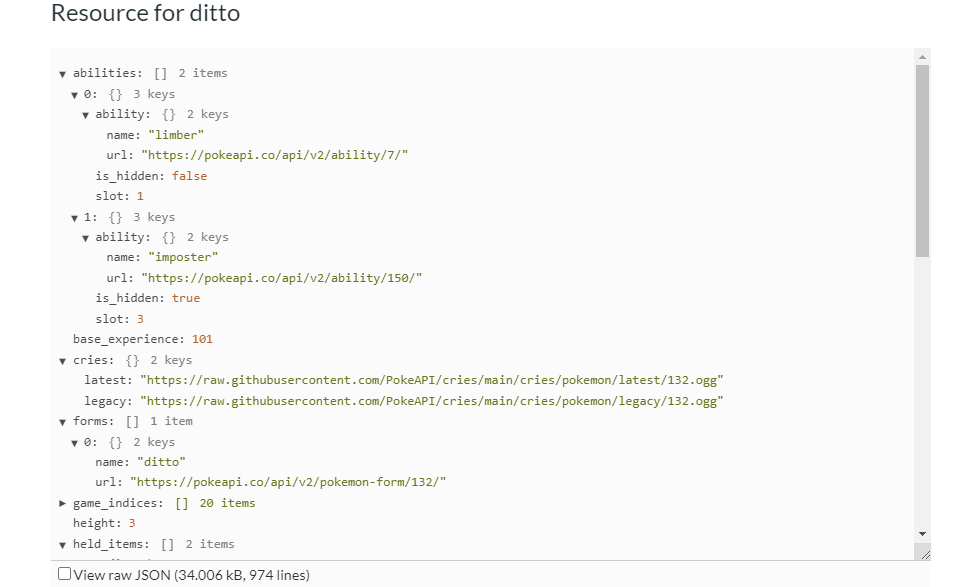
\includegraphics[width=0.4\textwidth]{images/API.png} % Reemplaza 'ruta/de/la/imagen' por la ruta de tu imagen
    \caption{Collider en JavaScript}
    \label{fig:mi_imagen}
\end{figure}



\subsection{Implementación Java Script}

Para la implementación del JS en este prototipo fue principalmente el uso de JQuery, Artyom y AJax, para iniciar con nuestra parte logica fue importante empezar con JQuery para poder añadir eventos a nuestro boton con el click pues esta libreria nos iba sintetizar codigo y ademas al momento de combinarla con AJAX nos facilia la comunicación con nuestra API para asi poder realizar la busqueda.

Una de las complejidades que usamos en nuestra parte logica fue traer los datos que se encontrban en diccionario, pero despues de investigación se puede dar cuenta que se puede traer <p></p> pues es una de la funcionalidades con HTML.

Para solucionar el problema con los diccionarios usamos esa misma función del HTMl solo que ahora añadimos{JSON.Stringify} para poder traer del API una ubicación exacta de nuestro diccionario que contenia un Array ademas de añadir condicionales para la mejor gestión de información.

Para implementar la busqueda de voz con la libreria Artyom fue una de las cosas que pense que eran complejas pero no lo eran, para la implementación de esta misma se intalo la libreria se inicializo y se empezo con la parte logica, buscamos que las plabras que se detectaban en consola fuera remplazada en mi barra de busqueda, para esto creamos una funcion combinado con un condicional, donde le añadimos "trim" y "toLowerCase", son herramientas que nos ayudan a ignorar la mayuscula y espacios, pues sin esto el manejo del error 404 siempre iba aparecer.

\begin{figure}[h] % Aquí comienza la inclusión de la imagen
    \centering
    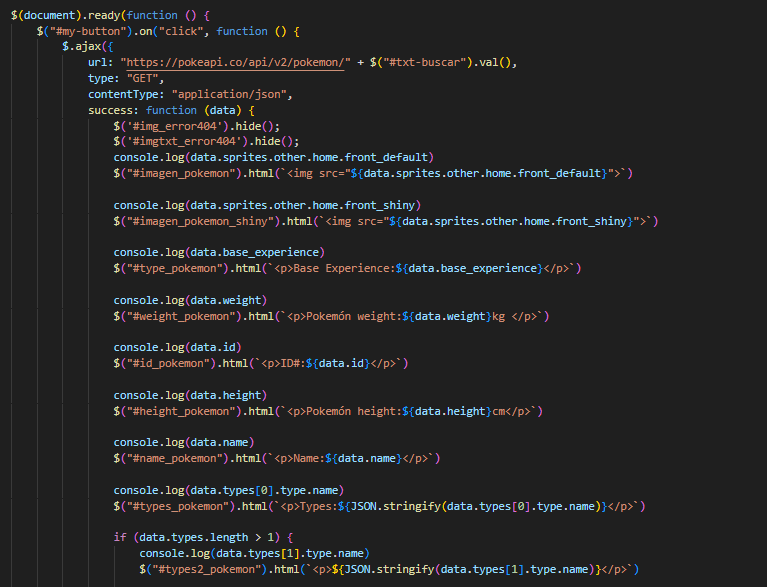
\includegraphics[width=0.4\textwidth]{images/JQuery.png} % Reemplaza 'ruta/de/la/imagen' por la ruta de tu imagen
    \caption{Implementación JQuery y AJAX}
    \label{fig:mi_imagen}
\end{figure}

\begin{figure}[h] % Aquí comienza la inclusión de la imagen
    \centering
    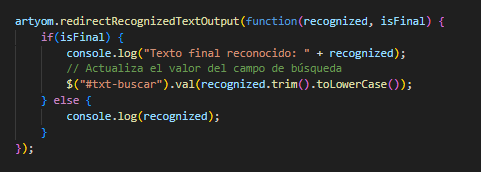
\includegraphics[width=0.4\textwidth]{images/ArtyomVoice.png} % Reemplaza 'ruta/de/la/imagen' por la ruta de tu imagen
    \caption{Implementación Artyom.js}
    \label{fig:mi_imagen}
\end{figure}

\subsection{Manejo del error 404}
Para el manejor del error fue unas de las cosas que tuvieron un grado de dificultad cuando se realizaban busquedas despues de aparecer el error, para poder solucionar este problema se uso JavaScript para que se esconda el error siempre que se encontrara y despues crear una funcion que haga que este error apareciera y ocultara los datos del Pokemon en cuestion.
\begin{figure}[h] % Aquí comienza la inclusión de la imagen
    \centering
    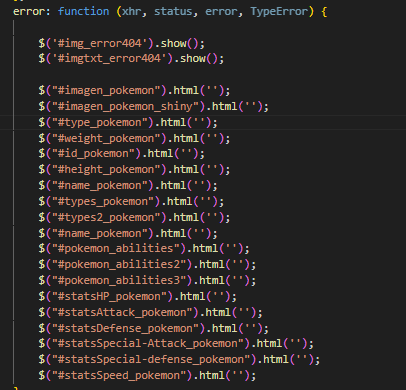
\includegraphics[width=0.5\textwidth]{images/Error 404 sh.png} % Reemplaza 'ruta/de/la/imagen' por la ruta de tu imagen
    \caption{Esconder Error 404}
    \label{fig:mi_imagen}
\end{figure}

\begin{figure}[h] % Aquí comienza la inclusión de la imagen
    \centering
    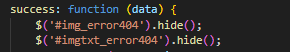
\includegraphics[width=0.5\textwidth]{images/error 404 show.png} % Reemplaza 'ruta/de/la/imagen' por la ruta de tu imagen
    \caption{Mostrar Error 404}
    \label{fig:mi_imagen}
\end{figure}

\subsection{Vista General del Prototipo}
En la vista general de mi protipo se logro realizar un pokewiki el cual sirve de consulta de los pokemones añadiendole busquedas de voz para dar mas opciones ha este prototipo ademas de los manejos de errores.

\begin{figure}[h] % Aquí comienza la inclusión de la imagen
    \centering
    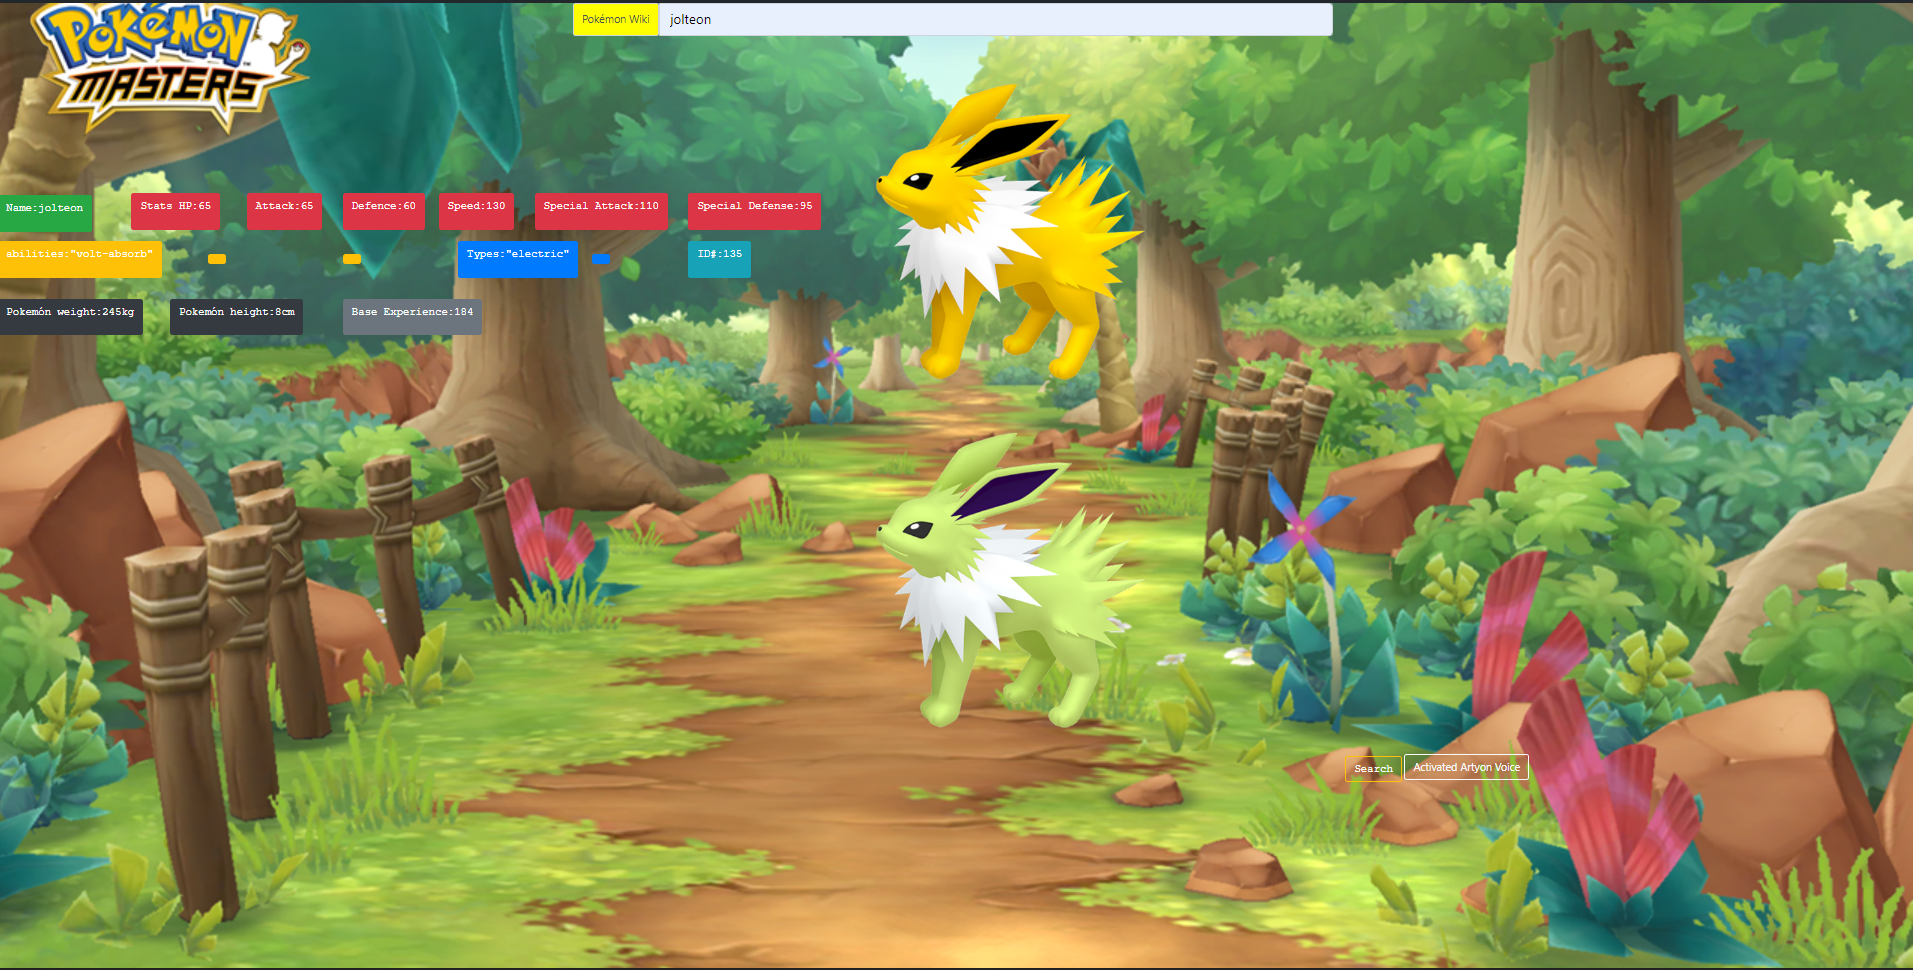
\includegraphics[width=0.5\textwidth]{images/PokeAPI View.png} % Reemplaza 'ruta/de/la/imagen' por la ruta de tu imagen
    \caption{Vista Final Del Prototipo}
    \label{fig:mi_imagen}
\end{figure}

\begin{figure}[h] % Aquí comienza la inclusión de la imagen
    \centering
    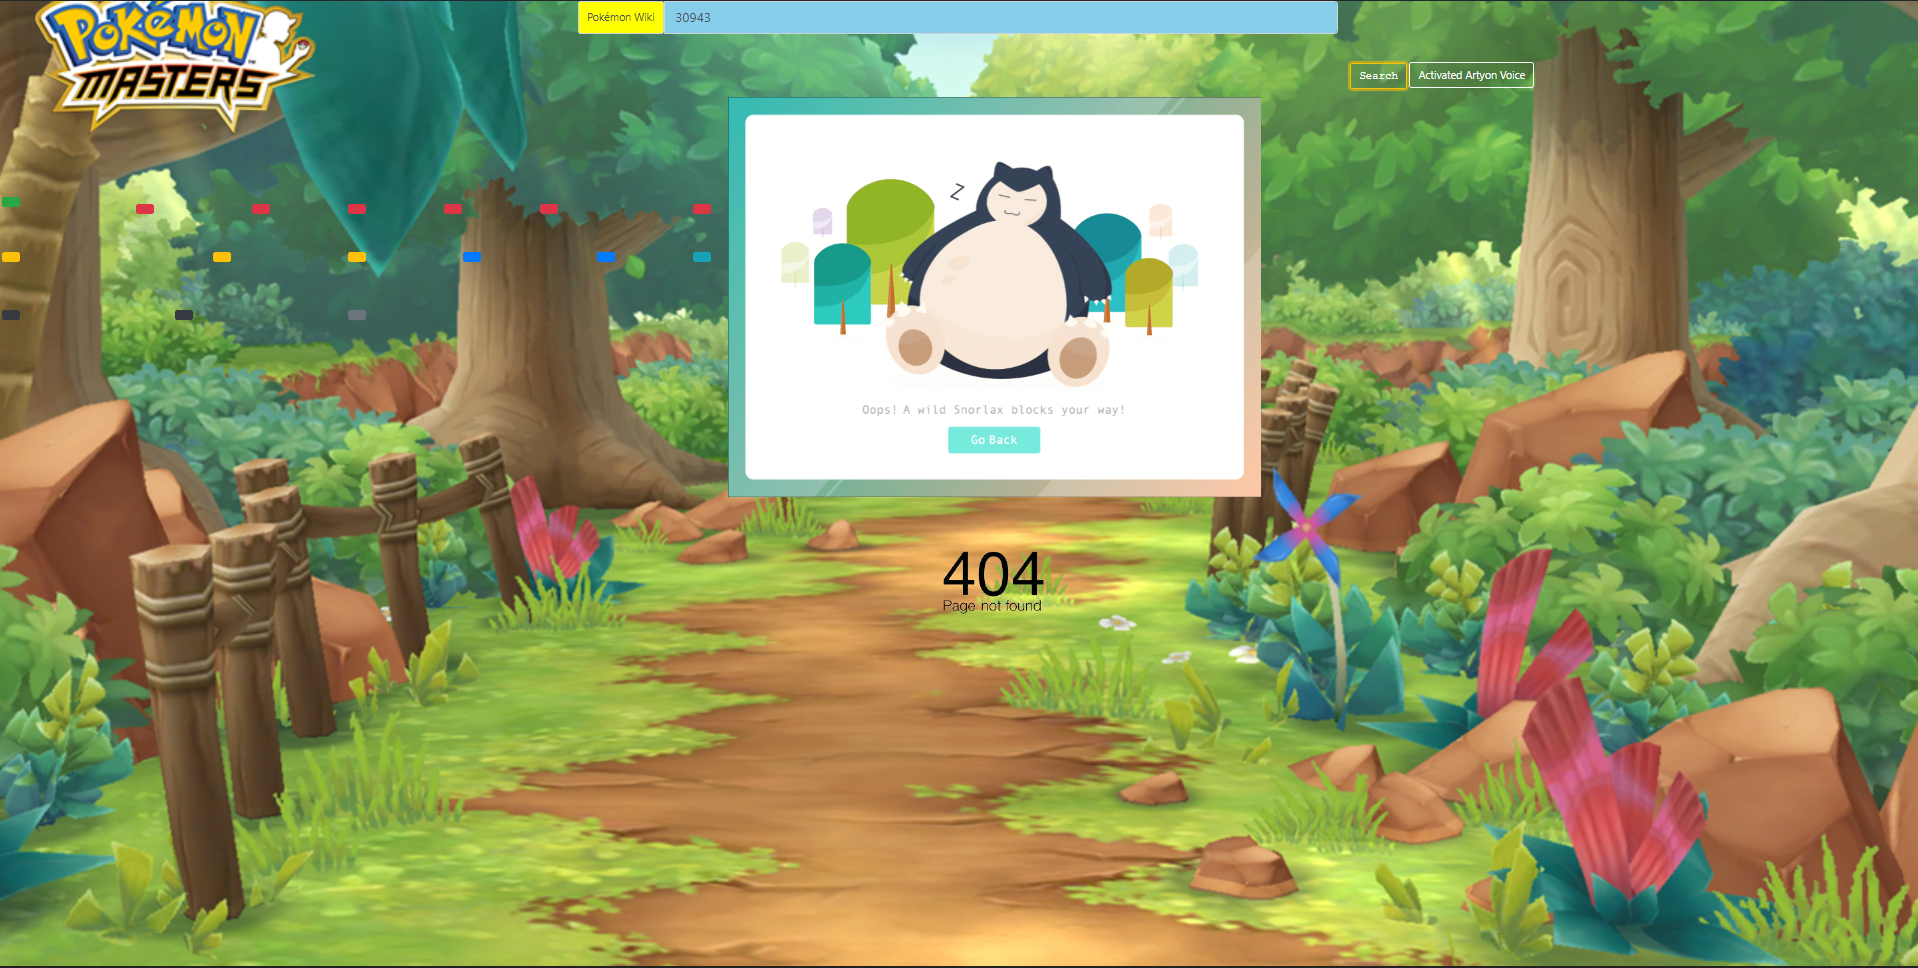
\includegraphics[width=0.5\textwidth]{images/Error 404 view.png} % Reemplaza 'ruta/de/la/imagen' por la ruta de tu imagen
    \caption{Vista Final Del Prototipo}
    \label{fig:mi_imagen}
\end{figure}

\subsection{Instructivo}
Para que el juego se pueda disfrutar en terminos general se debe ajustar siempre valores, para que el contenido se adapte a la pantalla y no se vea desproporcioando se pued eutilizar la combinacion de teclas "ctrl + +" o en su defecto "ctrl + -", estos valores son adaptables al gusto del usuario pero para resoluciones 1920 x 1080, el 67 porciento queda perfectamente ancajado.

Para la busqueda de voz es necesario tener un microfono funcional ademas de otorgar el permiso para que este pueda usar Artyom y por ultimo usar navegadores compatibles con Artyom como lo son Chrome o Edge.
\begin{figure}[h] % Aquí comienza la inclusión de la imagen
    \centering
    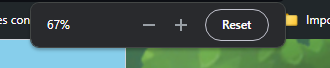
\includegraphics[width=0.5\textwidth]{images/67.png} % Reemplaza 'ruta/de/la/imagen' por la ruta de tu imagen
    \caption{Zoom para resoluciones 1920 x 1080}
    \label{fig:mi_imagen}
\end{figure}

\begin{figure}[h] % Aquí comienza la inclusión de la imagen
    \centering
    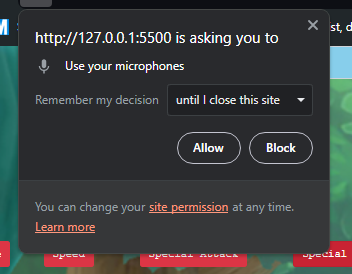
\includegraphics[width=0.4\textwidth]{images/Micro.png} % Reemplaza 'ruta/de/la/imagen' por la ruta de tu imagen
    \caption{Volumen recomendado}
    \label{fig:mi_imagen}
    \vspace{900pt} % Ajusta el espacio vertical aquí según tus necesidades
\end{figure}
\end{document}

